%% MATT2:  M. Peveler => M.\ Peveler, eg.  Need to propagate throughout the diss.

\chapter{INTRODUCTION, BACKGROUND, AND MOTIVATION}\label{chap:introduction}
\blfootnote{Portions of
  this chapter previously appeared as:
  \begin{itemize}[\indent { }]
  \item[] M. Peveler, N. S. Govindarajulu, S. Bringsjord, A. Sen, B. Srivastava,
K. Talamadupula, and H. Su, “Toward cognitive and immersive systems: 
Experiments in a cognitive microworld,” under review for \textit{Adv. in
Cogn. Syst.}, Stanford, CA, USA, Dec. 2020.
  \end{itemize}
 }

% 1. Introduction
\section{Introduction}

In contemporary AI research, especially as devoted to decision
support, the challenge is often taken to be that of providing AI
support to a single human on their own personal device. However, much
human problem solving is fundamentally social, in that a group of
people must work together to solve a problem, and must rely upon
machine intelligence that is itself highly diverse.  Examples of such
activities include: hiring a person into a university or company,
tackling an emergency crisis like a major water pipeline break,
planning an intricate medical operation, and deciding which companies
to merge with or acquire.  Motivated by such challenges, we are
interested in how an artificial agent --- embedded in a
social-collaboration environment like an immersive room --- can, on
the spot, help a group of human participants.

%%%%%%%%%%%%%%%%%%%%%%%%%%%%%%%%%%%%%%%%%%%%%%%%%%%%%%%%%%%%%%%%%%%%%%
\begin{figure}
\centering
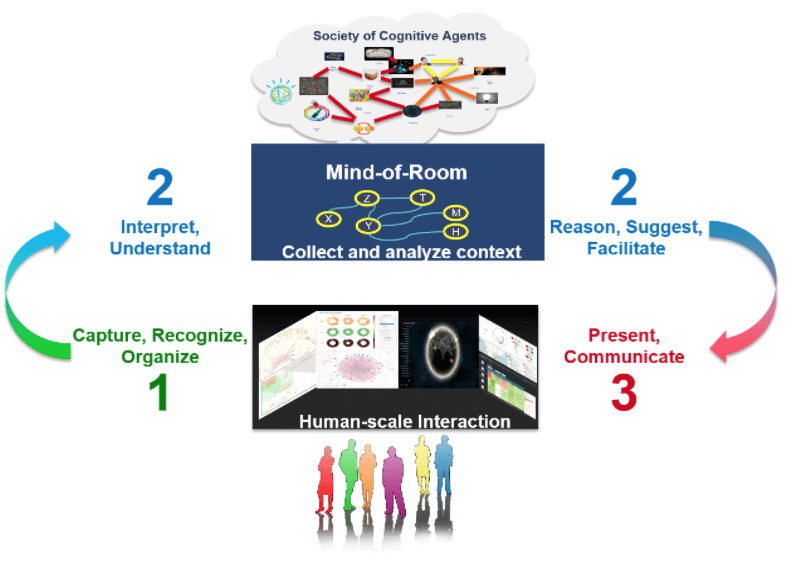
\includegraphics[width=0.5\columnwidth]{chapters/01_introduction/figures/cisl-cycle-graphic.png}
\caption{The flow of information through the elements of a cognitive and immersive system.}
\label{fig:cycle-cais}
\end{figure}
%%%%%%%%%%%%%%%%%%%%%%%%%%%%%%%%%%%%%%%%%%%%%%%%%%%%%%%%%%%%%%%%%%%%%%

We first introduce the notion of a \emph{cognitive and immersive
  system} (CAIS), which comprises three elements linked in a cyclical
flow as shown in Figure \ref{fig:cycle-cais}.  The first element is
responsible for perception and sensing within the environment that
contains the human agents (such as a room). Percepts come courtesy of
a range of sensors, such as microphones and kinects. From these
percepts, we receive information such as what was said, where users
are in the room, etc. The second element, upon receiving that
information, is responsible for interpreting, understanding, and
executing on the basis of that data. In this process, the CAIS may
employ reasoners, planners, databases, etc.\ to drive its
execution. The third element displays both percepts and the results of
processing these percepts in rich, multi-modal ways, such as showing
content on displays or speaking to the users of the system. As part of
the operation of the CAIS, we expect that it has access both to local
modules, as well as is able to make use of external machines and
services that are well-suited to specific tasks or domains. Perhaps
most important to note here is that these external services may be
requested for and opened by users of the system, but that one
reasonably expects that a CAIS should be able to handle these things
in a meaningful and useful fashion.
%% MATT2:  Previous sentence quite hard to understand.  Pls rework.
An important part of our system is that there are overseeing AIs
(agents) operating at the system level that can use the rest of the
system to assist and aid the humans and other AIs that are operating
within.  Thus, the overarching architecture is neither fully
centralized nor fully distributed, but aims to combine the strengths
of both.

Stemming from this overseeing AI, being that it captures all that goes
on within a CAIS, we can look to realize a number of useful
capabilities and principles. Most important here is that these stem
from a rigorous formalization, not from an \textit{ad hoc}
process. From these formal requirements and formalized operations, we
explore how this then also enables our CAIS to possess deeper levels
of understanding of human agents within the room, operating at a
proper theory-of-mind level~\cite{premack_does_1978}, and makes
capable automated means of reasoning, planning, and plan recognition.
An example of this is shown in the following section, and further
explored in Chapter~\ref{chap:planning}, utilizing reasoning to
determine the knowledge and belief of agents, and plan recognition of
what agents are attempting to accomplish to provide meaningful
assistance.

This dissertation is divided into three major parts. The first part
consists of this chapter and deals with the high level goals we lay
out for cognitive-and-immersive systems. We present a motivating
example, and discuss at a high-level abstract view what an idealized
CAIS may be able to accomplish. The second part of the dissertation
concerns mplementation of a real-world CAIS, focusing on two novel
compoments that allow us to to achieve mechanisms being multi-modal
and multi-user without having the system then be constrained to one
specific type of use case or domain. This part is encapsulated in
Chapters 2, 3, and 4. For the third part, which makes up Chapters 5
and 6, we now provide a formalization for these sorts of systems,
stemming from the implmentation in part 2, and then look to see how we
can utilize this for tasks in reasoning, planning, and plan
recognition. Finally, we conclude the work with a summary of our
contributions and recognize promising avenues of future work that
exist.


% 3. Motivating Example
\subsection{Motivating Example}

In this section, we provide an overarching motivating example to help
illuminate the challenges we hope to solve within this work. To help further
ground the work, we present an example that could be commonplace within a joint
meeting space, and does not include a contrived setup.

Imagine that within a CAIS, there are three humans, Alvin, Betty, and Charlie,
who are all jointly working on a shared problem. Alvin and Betty are standing
next to each other, while Charlie stands apart. There is content on the screen
that relates to the problem. Betty looks at Alvin, then points at a particular
region of the screen. Alvin, seeing that Betty is looking at him, looks at her,
then follows to where she is pointing at the screen. Charlie is not looking at
either Alvin or Betty, nor at the region of screen that Betty is pointing at,
but instead at some other region of the screen. Betty gestures at the region of
the screen that she is pointing at, and the content changes in some way. Alvin,
who is following along the pointing and gesture, perceives both the gesture, and
the content change on the screen, while Charlie does not. Alvin then points to
the screen and makes a gesture, changing the content on the screen for a second
time. Betty perceives the pointing and gesture that Alvin does, while Charlie is
still oblivious to it. The time for this meeting concludes, and Betty might
reasonably ask "is everyone on the same page?". Neither Alvin or Betty are aware
that Charlie is not, while Charlie is unaware of the changed content. The
CAIS steps in, saying that no, Charlie is not on the same page, and that here
is a summary of the actions of Alvin and Betty for Charlie to catch him up,
covering the content that Alvin and Betty had both pointed at, as well as
the content that had changed on the screen.

From this example, we see that the CAIS must possess a number of sophisticated
pieces of machinery. For the physical space, the CAIS must possess the capacity
of knowing who is using the system, the physical actions that they
undertake, and what these agents might say. The CAIS then must possess the
capacity to display information to the human participants and speak to the
human participants. Finally, the CAIS must be able to connect the physical
actions of the humans, to that of the content that is being shown within the
space, such that it connects Betty gesturing at the screen with content under
that gesture.


% 2. Requirements of a CAIS
\section{Requirements of CAIS}\label{ref:requirements_cais}

It should be noted that for a CAIS to be considered a truly
``intelligent'' room, it is not sufficient that the room be
intelligent about, for example, search queries over a domain $D$; the
room should also be intelligent about cognitive states of agents in
the room and their cognitive states towards $D$.

Despite there being a significant amount of work done in building
intelligent environments (of varying levels of intelligence;
\cite{coen_design_1998,brooks_intelligent_1997,chan_review_2008}),
there is no formalization of what constitutes an intelligent room and
what separates it from an intelligent agent.  Though
\cite{coen_design_1998} briefly differentiates an intelligent room
from ubiquitous computing based on the non-ubiquity of sensors in the
former, there is not any formal or rigorous discussion of what
separates an intelligent room from a mobile robot that roams around
the room with an array of sensors. As far as we are aware, this work
is novel in its act of providing a characterization of what separates
an intelligent room from an intelligent agent.

The requirements in question are cognitive in nature and exceed
intelligent rooms with sensors that can answer queries over simple
extensional data (e.g.\ a room that can answer financial queries such
as \textit{``Show me the number of companies with revenue over X?''}).
At a high-level, we require two conditions below hold:

\begin{itemize}
    \item $\mathcal{C}$ \emph{Cognitive}: A CAIS should be able to
      help agents with cognitive tasks and goals.  For instance, a
      system that simply aids in querying a domain $D$ is not
      cognitive in nature; a system that knowingly aids an agent in convincing
      another agent that some state-of-affairs holds in $D$ is
      considered cognitive. (Please see the appendix for more
      discussion of our usage of the term ``cognitive.'')
    \item $\mathcal{I}$ \emph{Immersive}: There should be some
      attribute or property of a CAIS that is non-localized and
      distinguished from agents in the room.  Moreover, this property
      should be \textbf{common knowledge}.\footnote{For our purposes,
        common knowledge as defined in Chapter~\ref{chap:formalizing}
        is that all agents know this property, and know that all other
        agents know it.}  (Note: this is not easily achievable with a
      physical robot, and this condition differentiates a CAIS from a
      cognitive agent.)
\end{itemize}

While we believe that $\mathcal{C}$ is fully realizable and is
achieved as part of this dissertation, $\mathcal{I}$ is certainly far
more ambitious, given the high level of sophistication necessary for
an implementation that satisfies this condition. As such, we posit
that for a true formalization to hold any water, it must stem from the
implementation and not vice versa. In this way, we can ground our
formalization in a working system that can properly showcase both the
formalization and our technology.

\begin{comment}
\footnote{This condition may not strictly be realizable,
        but the goal is to at a minimum build systems that approach
        this ideal condition.}
\end{comment}


% 1. Overarching Goals


% 4. Colocated vs Distributed

\section{On Co-location vs Distributed Usage}

Before continuing, we would like to take a moment to discuss the
beliefs of co-location vs distributed usage of these sorts of
technologies. Within this work, we present, and focus on, a vision of
how such systems can be applied and help with co-located
participants. While we do believe that elements of this work can be
applied to a digital domain, doing so fundamentally changes the
paradigm of collaboration. When working together, we use the humans
%% MATT2:  "use the humans"?  Not sure what is meant here.  Pls
%% clarify, refine.  Thx.
utilize different levels of coupling, increasing or decreasing based
on the extent of communication that is required by the task at
hand~\cite{salvador_denver_1996,olson_distance_2000}. However, it is
important that coupling is not a static concept through a task, rather
that it is dynamic, changing through the lifetime of a
task~\cite{jakobsen_up_2014}.  Within this coupling, we see rise to a
concept of ``we-awareness" amongst
participants~\cite{greenberg_implications_2016}, as they utilize some
level of implicit understanding of verbal and non-verbal
communications. These concepts do not easily transfer to distributed
digital systems wherein participants are no longer standing next to
each other, rather sharing a ``space'' through interfaces like video
chat. Take for example pointing to something on a screen. With two
people standing next to each other, and one pointing at a shared
screen, we can make reasonable assumptions regarding the cognitive
states of agents, what they're perceiving, and also regarding what
they might believe about each other and what each other perceives.

Moving to the digital realm, these concepts cannot be immediately
recast as is, as one must first design the necessary mechanisms to
capture that information, transmit it to the other participants, and
to do so in such a way that the many rich and subtle parts of that
face-to-face interaction are not lost. Given the complexity of that
task, and the research area unto itself it would require, we do not
attempt to give the parallels here; we instead focus just on the topic
of handling the work in the co-located version only.


% 5. Contributions of the Dissertation

\section{Proposed Contributions of the Dissertation}

We now lay out the novel contributions of this work:

\begin{enumerate}
\item Create a high-level but rigorous and fertile definition for what
  constitutes a CAIS, separating it from a physical robot.
\item Define a framework for how one approaches building a CAIS.
\item Create a real-world implementation of a CAIS, demonstrating at a
  novel level that it:
        \begin{enumerate}
            \item adapts to a number of potential input mechanisms;
            \item operates at a true multi-modal and multi-user level; and
            \item is capable of interacting with and understanding
              third-party content.
        \end{enumerate}
      \item Create a formal definition of a CAIS' implementation and
        its capabilities.
      \item Utilize the above items to handle tasks of reasoning,
        planning, and plan recognition in and involving a CAIS.
\end{enumerate}
